\section*{Inverses as reflections}

\begin{myConceptSteps}{To see the visual relationship between a function and its inverse\dots}
    \myStep{original function}{Sketch the graph of the original function $y = f(x)$.}
    \myStep{inverse function}{Sketch the graph of the inverse function $y = f^{-1}(x)$.}
    \myStep{diagonal}{Lightly sketch the graph of the diagonal line, $y=x$ (or draw it as a dotted line).}
    \myStep{notice}{
        Notice that the graph of the inverse function 
        is the mirror image (reflection) of the original function 
        across that diagonal line.    }
\end{myConceptSteps}


\begin{myExample}{\( f(x) = x^5 \)}
    Let's consider the function 
    \( f(x) = x^5 \).
    It turns out (we will learn this later in the year)
    that the inverse of this function its
    \( f^{-1}(x) = \sqrt[5]{x} \).
    \vskip1em
    We could (but you {\bfseries\itshape do not} need to) use a graphing calculator or Desmos to graph $f$ and $f^{-1}$:

    \begin{center}
    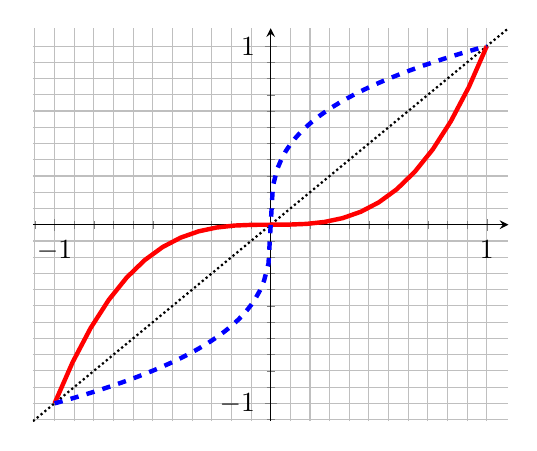
\begin{tikzpicture}
    \begin{axis}[
        width=3in,
        grid=both,
        axis x line = middle,axis y line = middle,
        % axis equal image,
        xtick distance = 1, ytick distance = 1,
        minor tick num=10,
        ]
        \addplot[no marks,densely dotted,thick,domain=-1.1:1.1]{x};
        \addplot[no marks,solid,red,ultra thick,domain=-1:1]{x^3};
        % cube root, see: https://tex.stackexchange.com/questions/69411/pgfplots-cant-plot-some-usual-mathematical-functions
        \addplot[no marks,solid,blue,dashed,ultra thick,domain=-1:1,samples=100]{x/abs(x)*abs(x)^(1/3)};
    \end{axis}
    \end{tikzpicture}
    \end{center}
    
    \noindent Notice how the two graphs are {\bfseries\itshape mirror images} of each other 
    across the diagonal line.
\end{myExample}


\begin{taggedblock}{on-level}
    \begin{myExample}{Sketch the graph of the inverse of the function shown below.}
        The grid below contains the graph of the function $f(x) = \frac{1}{2}x$. 
        Based on what you have learned about \emph{inverses} and \emph{mirror images},
        sketch the graph of the inverse function.

        \begin{center}
            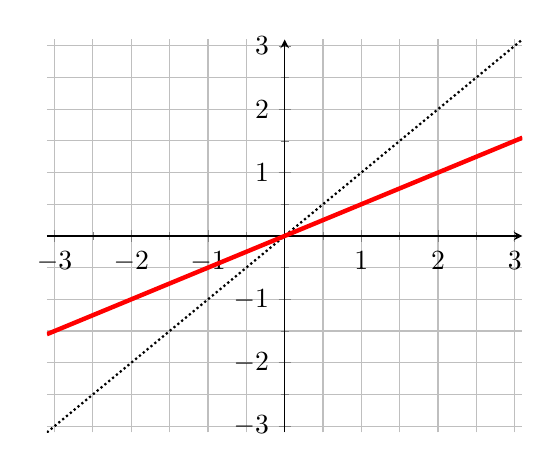
\begin{tikzpicture}
            \begin{axis}[
                width=3in,
                grid=both,
                axis x line = middle,axis y line = middle,
                % axis equal image,
                xtick distance = 1, ytick distance = 1,
                minor tick num=1,
                ]
                \addplot[no marks,densely dotted,thick,domain=-3.1:3.1]{(x};
                \addplot[no marks,solid,red,ultra thick,domain=-3.1:3.1]{(1/2)*x)};
            \end{axis}
            \end{tikzpicture}
        \end{center}
    \end{myExample}
\end{taggedblock}



\begin{taggedblock}{pre-AP}
    \begin{myExample}{Sketch the graph of the inverse of the function shown below.}
        The grid below contains the graph of the function $f(x) = 2^x$. 
        Based on what you have learned about \emph{inverses} and \emph{mirror images},
        sketch the graph of the inverse function.

        \begin{center}
            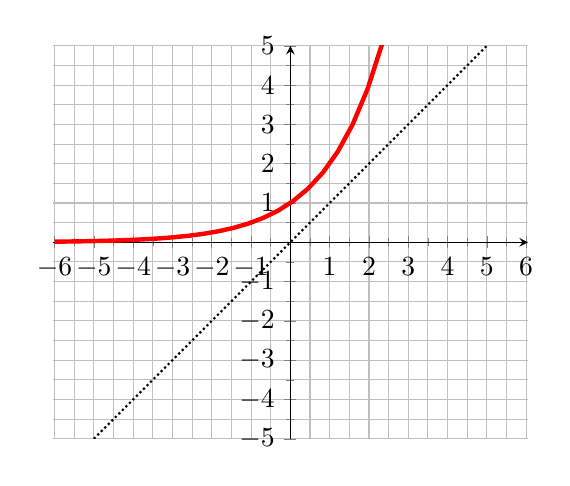
\begin{tikzpicture}
            \begin{axis}[
                width=3in,
                grid=both,
                axis x line = middle,axis y line = middle,
                % axis equal image,
                xtick distance = 1, ytick distance = 1,
                minor tick num=1,
                axis equal,
                ymin = -5, ymax = 5,
                xmin = -5, xmax = 5,
                ]
                \addplot[no marks,densely dotted,thick,domain=-5:5]{(x};
                \addplot[no marks,solid,red,ultra thick,domain=-6:3.1]{2^x)};
            \end{axis}
            \end{tikzpicture}
        \end{center}
    \end{myExample}    
\end{taggedblock}